\documentclass{article}

% packages
\usepackage{listings}
\usepackage{graphicx}
\usepackage{xcolor}
\usepackage{inconsolata} % Modern monospace font
\usepackage{hyperref} % for linking sections in text

% === Basic Syntax Highlighting ===

% \definecolor{codegreen}{rgb}{0,0.6,0}
% \definecolor{codekeyword}{rgb}{0.86,0.24,0.62}
% \definecolor{codegray}{rgb}{0.5,0.5,0.5}
% \definecolor{codepurple}{rgb}{0.58,0,0.82}
% \definecolor{codebackground}{rgb}{0.95,0.95,0.92}

% \lstdefinestyle{mystyle}{
%     backgroundcolor=\color{codebackground},   
%     commentstyle=\color{codegreen},
%     keywordstyle=\color{codekeyword},
%     numberstyle=\tiny\color{codegray},
%     stringstyle=\color{codepurple},
%     basicstyle=\ttfamily\footnotesize,
%     breakatwhitespace=false,         
%     breaklines=true,                 
%     captionpos=b,                    
%     keepspaces=true,                 
%     numbers=left,                    
%     numbersep=5pt,                  
%     showspaces=false,                
%     showstringspaces=false,
%     showtabs=false,                  
%     tabsize=2
% }

% =================================

% --- Tokyo Night Light Palette ---
\definecolor{tnBackground}{HTML}{e1e2e7}  % Main background
\definecolor{tnText}{HTML}{343b58}        % Base text / identifiers
\definecolor{tnComment}{HTML}{9699a3}     % Comments
\definecolor{tnKeyword}{HTML}{7847bd}     % Keywords (purple)
\definecolor{tnString}{HTML}{485e30}      % Strings (dark green)
\definecolor{tnFunction}{HTML}{0f4b6e}    % Functions / Methods (blue)
\definecolor{tnNumber}{HTML}{8c4351}      % Numbers / Constants (red/burgundy)
\definecolor{tnOperator}{HTML}{005af0}    % Operators (cyan/blue)
\definecolor{tnLineNum}{HTML}{9699a3}     % Line numbers

% --- Define Tokyo Night Light Style ---
\lstdefinestyle{tokyonight-light}{
    backgroundcolor=\color{tnBackground},
    basicstyle=\ttfamily\small\color{tnText},
    commentstyle=\color{tnComment}\itshape,
    keywordstyle=\color{tnKeyword}\bfseries,
    stringstyle=\color{tnString},
    numberstyle=\tiny\color{tnLineNum},
    identifierstyle=\color{tnText},
    breakatwhitespace=false,
    breaklines=true,
    captionpos=b,
    keepspaces=true,
    numbers=left,
    numbersep=10pt,
    showspaces=false,
    showstringspaces=false,
    showtabs=false,
    tabsize=4,
    frame=single,
    rulecolor=\color{tnBackground},
    framerule=0pt,
    framexleftmargin=6pt,
    framexrightmargin=6pt,
    framextopmargin=6pt,
    framexbottommargin=6pt
}

\lstset{style=tokyonight-light}

\title{Contributing to KDEEcoLab - Systematic Measurement of Software Energy Consumption}

\begin{document}

    % turn off pagenumbering
    \pagenumbering{gobble}
    \maketitle
    \newpage

    \tableofcontents

    \newpage

    \section{About KDE and the KEcoLab project}
        \textbf{What is KDE?}
        \newline
        KDE is a very well known international software community, well known for example for the Plasma desktop, but also for many other programs, like Kate, KDevelop, etc.

        \subsection{About KEcoLab - the current project status and the goals}
        \textbf{What is KEcoLab?}

    \section{Get familiar with the project}

        \subsection{KEcoLab repository}
        \textbf{What's inside of the repository? (structure, actual code, etc.)}

        \subsection{ydotool, kdotool and xdotool - Actual problems}
        \textbf{How does ydotool work? Pros, Cons?}

        \subsection{The scripting scenarios}
        \textbf{Description of the scenarios, what are the steps, which are done}

        \subsubsection{Baseline scenario}
        \subsubsection{Idle Scenario}
        \subsubsection{System Usage Scenario}

        \subsection{Setting up the environment}
        \textbf{What is the working setup generally?}
        \subsubsection{Fedora VM with KDE Plasma}

        \begin{lstlisting}
         sudo dnf upgrade
        \end{lstlisting}

        \subsubsection{Setup ydotool and kdotool}
        To run the actual scripts, also kdotool and ydotool have to be set up, as the scripts are built on these programs. So first for the installation make sure, to also have cmake, g++/clang and sdoc installed. If not, install them(in this example g++ is used, to install clang just swap g++ with clang):
        \begin{lstlisting}
         sudo dnf install cmake g++ scdoc
        \end{lstlisting}

        Further clone the repository and install the application by using:
        \begin{lstlisting}
         git clone -b feat/setup-script https://invent.kde.org/neogg/ydotool.git
         cd ydotool
         chmod +x setup.sh
         ./setup.sh install
        \end{lstlisting}

        Also give ydotoold persmissions to uinput:
        \begin{lstlisting}
         sudo touch /etc/udev/rules.d/99-uinput.rules
         echo 'KERNEL=="uinput", MODE="0660", GROUP="input"' | sudo tee /etc/udev/rules.d/99-uinput.rules > /dev/null
         sudo usermod -aG input "$USER"

         sudo udevadm control --reload-rules
         sudo udevadm trigger
        \end{lstlisting}

        Now the system has to be rebooted and after that ydotool can be started by using:
        \begin{lstlisting}
         systemctl --user start ydotoold
        \end{lstlisting}

        To verify, that everything worked you can try some ydotool commands, as example lets try to do the bash command ls via the  ydotool interface:
        \begin{lstlisting}
         ydotool type "ls" && ydotool key 28:1 28:0
        \end{lstlisting}
        This types "ls" to the command-line and key does press keys - 28 stands for enter, 0 is release and 1 is press.

        A keymap where all keys are described can be found in `/usr/include/linux/input-event-codes.h`.

        \textbf{!!!MISSING KDOTOOL!!!}
        \newline

        \subsection{Run the project locally and test the scripts}
        Now that the VM is setup and ydotool/kdotool are installed, it can be tried to run the actual scripts. As the script of Okular is the only script, which is working, those will be run. First, the KEcoLab repository has to be cloned locally by using:
        \begin{lstlisting}
         git clone https://invent.kde.org/sdk/kecolab.git
        \end{lstlisting}
        This will create the project folder, in order to be able to access the scripts. These are stored in `scripts/test\textunderscore scripts/org.kde.okular`. The folder contains three scripting files, one for each scenario.
        To be able to run the scripts you need the flatpak version of the application. As this script is now for Okular, the `org.kde.okular` package
        needs to be installed by running `flatpak install org.kde.okular`.
        If not installed, the script is not able to start the application.
        Also the scripts have to be executable, which is done by `chmod u+x $<$file-name$>$`. After these steps the script can be started and will run.
        For example starting the idle script would be `./log\textunderscore idle.sh`

        The scripts have principially the same structure until it comes to the testing for-loop. Each one has a syncUp-function defined, which sets sleep for the given time.
        `startAction()` and `stopAction()` will log the exact time of each action's start and stop to `~/log\textunderscore usage\textunderscore scenario`, as each action is wrapped with both functions. These functions are only defined in sus and idle scenario, as with baseline-scenario it's not needed.
        \subsubsection{Baseline scenario}
        This scenario is the most simple one, as there's not application started or anything else done, than logging the time of each iteration's start/end and waiting for 218s (including burn-in time of 60s and cooldown of 30s)
        \subsubsection{Idle Scenario}
        The idle scenario additionally contains the start of the application. Furthermore it will let Okular run for 220 seconds and then close it, which makes the scenario of the plain application running, with no actions done.
        \subsubsection{System usage Scenario}
        For running the system usage scenario, the configuration of the following key-shortcuts have to be made, as ydotool does many operations using shortkeys:
        \begin{itemize}
         \item Rotate Left: Ctrl+l
         \item Rotate Right: Ctrl+r
         \item Invert color: Ctrl+i
         \item Fit to width: Ctrl+Shift+w
         \item Single page mode: Ctrl+Alt+s
        \end{itemize}
        Also make shure that ydotool is running.
        The lines until the main for-loop are basically the same as in the idle script. For simulating the usage, a PDF-file is needed. The existance of a testing file is checked during the script at the beginning, and downloaded, if the file is not at the specified path. As the for loop starts, the pdf gets copied to the home directory:
        \begin{lstlisting}
         cp ~/Documents/okular/20yearsofKDE.pdf ~/Documents/20yearsofKDE
        \end{lstlisting}
        After copying the file and a wait time of 60s the file gets opened with:
        \begin{lstlisting}
         flatpak run org.kde.okular ~/Documents/20yearsofKDE > /dev/null 2>&1 &
        \end{lstlisting}
        `/dev/null 2$>$\&1 \&`suspends the output, so no output is given to the command line.

        \subsection{Change the source code and perform a merge request}

    \newpage
    \section{Selenium}
        \subsection{Why Selenium?}
        \textbf{What are the benefits compared to the actual scripts? 
        Would there be other solutions/frameworks? Etc...}

        \subsection{Setting up Selenium}
        As Selenium is designed to work and test within web browsers, our setup 
        needs some extra components.\\
        Thankfully we already have a solution in the form of KDE's "at-spi" 
        accessability api.

        \subsubsection{Overwiew}
        \textbf{Selenium} A Browser automation framework.\\
        \textbf{Driver} The server component of Selenium.\\
        \textbf{Appium} An extension to Selenium making it more useful for app 
        testing.\\
        \textbf{AT-SPI2} A protocol over DBus, which GUI toolkit widgets use to 
        provide their content to screen readers.\\

        \subsubsection{Installing Dependencies}
        Some or most of the following packages might already been installed on 
        the fedora distro, but to make sure, we will run the install commands 
        through our package manger.
        \begin{itemize}
            \item a supported Python3 version
            \item at-spi2
            \item pyatspi2
            \item accerciser
            \item gobject-introspection
        \end{itemize}
        We are gonna install these and other dependencies through our package 
        manager ("DNF" on fedora):
        \begin{lstlisting}[language=bash]
            sudo dnf install \
            at-spi2-core \
            accerciser \
            gobject-introspection \
            python3 \
            python3-pip \
            python3-pyatspi \
            python3-gobject \
            at-spi2-core \
            accerciser \
            cairo-devel
        \end{lstlisting}
        Additionally we ar going to need to install the following packages:
        \begin{lstlisting}[language=bash]
            sudo dnf install gcc \
            gobject-introspection-devel \
            cairo-gobject-devel \
            pkg-config python3-devel \
            gtk4
        \end{lstlisting}
        Including the following in order to be able to build 
        "selenium-webdriver-at-spi" in the following steps.
        \begin{lstlisting}[language=bash]
            sudo dnf install \
            extra-cmake-modules \
            qt6-qtbase-devel \
            qt6-qtbase-private-devel \
            qt6-qtdeclarative-devel \
            kf6-kwindowsystem-devel \
            plasma-wayland-protocols-devel \
            kwayland-devel \
            kpipewire-devel \
            kwin-devel \
            wayland-devel \
            ruby
        \end{lstlisting}
        Once we have these packages installed we are now ready to clone and 
        install selenium.

        \subsubsection{Installing Selenium-webdriver-AT-SPI}
        \begin{lstlisting}
            git clone https://invent.kde.org/sdk/selenium-webdriver-at-spi.git
            cd selenium-webdriver-at-spi
            # For virtual environment
            python3 -m venv --system-site-packages venv
            source venv/bin/activate
            pip3 install -r requirements.txt
            echo export PATH="~/.local/bin:$PATH" >> ${HOME}/.bashrc
            mkdir build
            cd build
            cmake ..
            make
            sudo make install
            cd ..
        \end{lstlisting}
        Now that Selenium is built, it can be used to run the Selenium-specific test.

        \subsubsection{Running Selenium Tests}
        If we are running our tests inside a VM -- which we do when working 
        with the scripts locally --, we make sure to set it up properly.\\
        In this case we are using QEMU/KVM Virtual Machine Manager.\\

        In the VM's settings, we go to the video tab and make sure 
        the Mode is set to Virtio and that 3D acceleration is checked.\\
        Then under Display Spice we need to make sure OpenGL is checked and 
        listen type is set to None.\\

        Now that the VM is set up and after rebooting the guest machine, we 
        will be able to run the Selenium tests.
        In order to test if it works we can run the example test by using the 
        following command from the selenium folder.

        \begin{lstlisting}
            selenium-webdriver-at-spi-run ./examples/calculatortest.py
        \end{lstlisting}
        If everything is working correctly, a window will open in which the 
        KCalc app will open and the test will run.

        \subsubsection{Using already existing Selenium scripts}
        Given an KDE-repository containing Selenium tests scripts for KDE Linux with OpenQA, it will be checked, if these scripts are of any further use for the current project.
        The repository https://invent.kde.org/kde-linux/os-autoinst-distri-kdelinux/-/tree/master/tests has the following structure:
        \begin{lstlisting}
         tests/
            common/
            kdelinux/
            kdelinux-live/
        \end{lstlisting}
        Each folder contains tests for different cases. The repository defines three test suites:
        \begin{itemize}
         \item install-system
         \item upgrade-system
         \item sanity-test
        \end{itemize}
        Each test-suite contains multiple tests, but most of them are for the os, like for example booting the system.
        Though in 'kdelinux/app/' there are some scripts, which could be useful for this work.
        First there is 'firefox.py':

        \begin{itemize}
         \item shebang, chmod u+x firefox.py
         \item create venv, install unittest-xml-reporting
         \item copy lib folder to where the script lies (!!find workaround!!)
         \item
         \item
         \item
        \end{itemize}


        Follow steps from \#\# Run tests locally - install podman-compose


%     \section{Transfer scripts to the target framework Selenium for each application and test-case}
%         \subsection{Baseline, Idle, Standard Usage Scenario}
%         \subsubsection{Okular}
%         \subsubsection{Kate}
%         \subsubsection{LibreOffice}
%
    \section{Testing software by setting up a Lab}

    To do own measurements on programm's energy consumption, a new testing Lab will be set up. As far as possible, the criteria of Blue Angel are followed, but due to the range of this project, it is not possible to arrange every point of the needed circumstances.
    In the following chapter the whole measuring process will be described, as well as which tech-stack and software is needed. The main goal is to show the differences of energy consumption between programs.


        \subsection{Software and Hardware requirements for the lab setup}
        For performing real software test, a few preparatios have to be made. The most important components to reach that are the power meter and two PCs, the first one for Processing the data and the second one for running the scripts with the three usage scenarios (KDE Eco Handbook).
        The following image, created by Lana Lutz (KDE) gives a good overview:

        \begin{figure}[h]
        \centering
        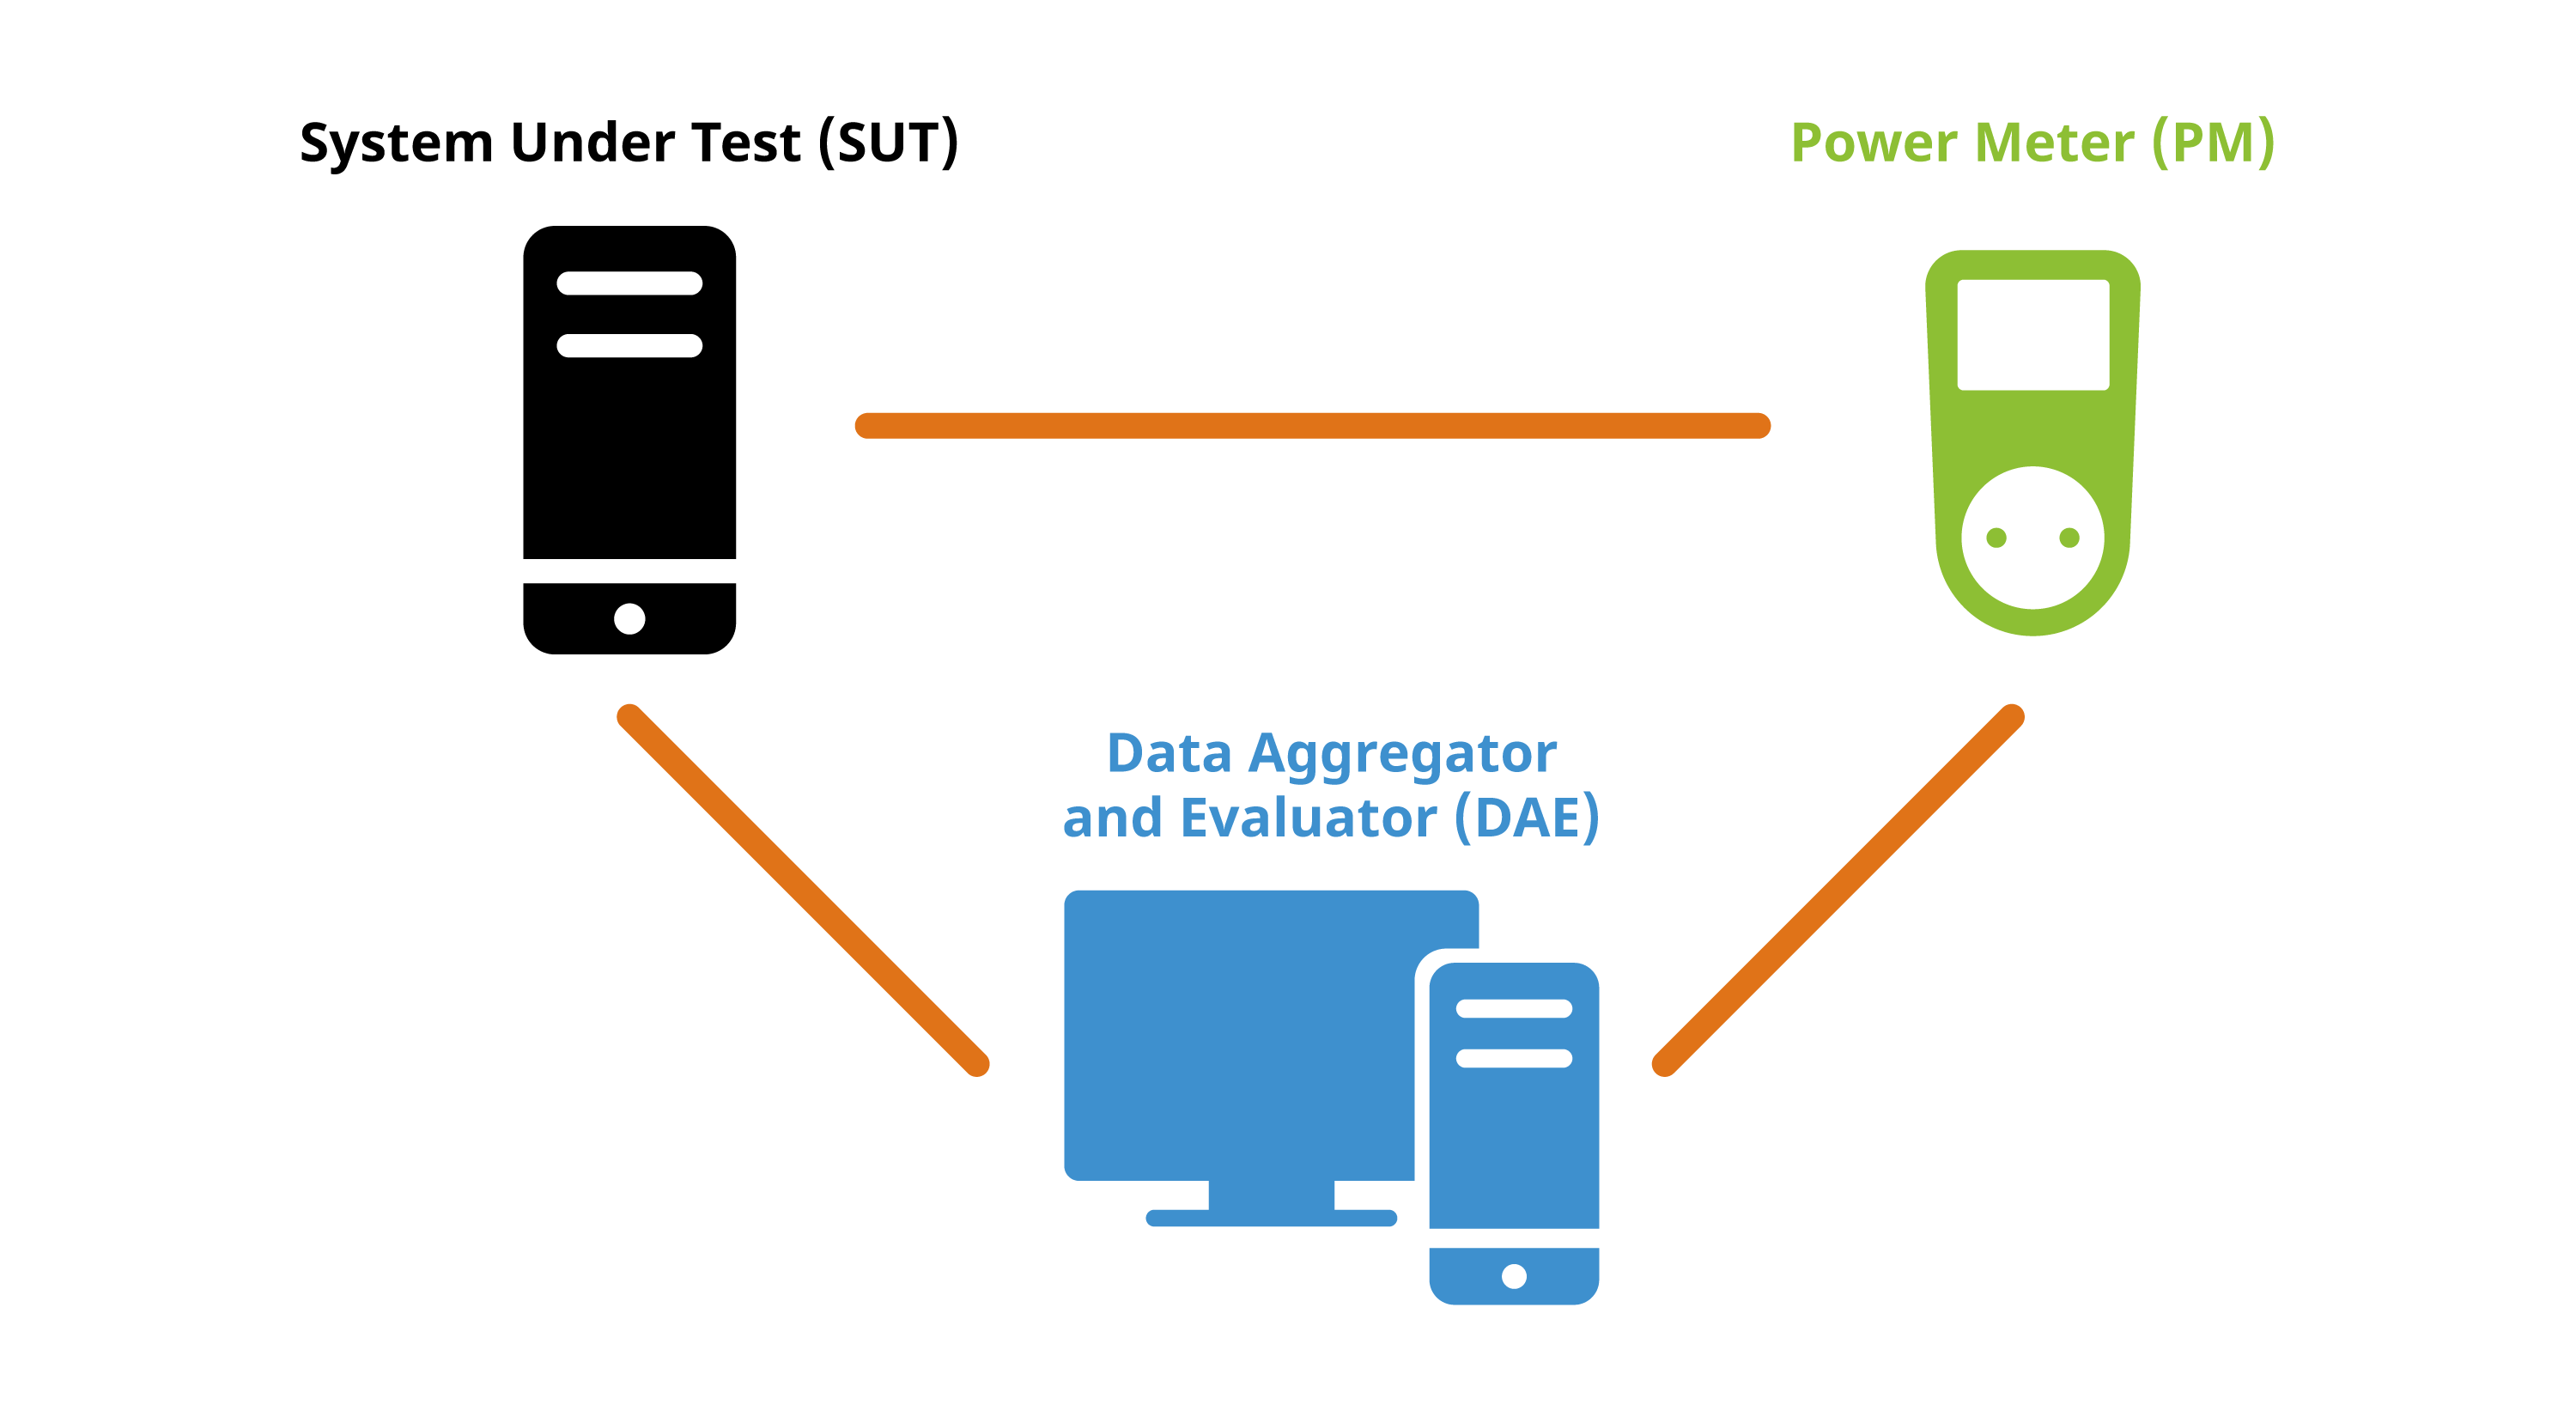
\includegraphics[width=10cm]{../img/sec3_lab-setup_modified.png}
        \end{figure}

        \subsubsection{Power meter}\label{power meter}
        First, to measure the energy consumption of anything, a power meter is needed. This will be provided by the school and is of the brand Sirius. The device which is recommended by Blue Angel is the 'Gude Expert Power Control 1202 Series'. The power meter should at least do one measurement per second and also create additional system logs with timestamps. To create these logs, the recommended tool is 'Collectctl'. This tool logs system relevant data, like RAM usage, CPU loading, or network status (Blauer Engel, S. 36).
        The data, which is collected, has to be stored in CSV format. One of the benefits is, that KDE's 'LabPlot' can process the CSV data live to output the data. Still, the main reason for storing the data into CSV is, that the analysis tool OSCAR, which is provided by the Campus Birkenfeld, needs this format (KDE Eco Handbook).
        \subsubsection{Data Aggregator and Evaluator}
        The next part is a PC as Data Aggregator and Evaluator is needed, which collects and processes the data from the power meter. The recommended power meter of Blue Angel can be used with a Python script, to read out the measurement. The device used for this lab comes with it's own proprietary software. Using this would cross the ethical principles of KDE, as it is no free open source software and further is not available for Linux. Due to this the open source solution 'openDAQ' will be used, which can be used combined with C++ or Python.
        \subsubsection{System Under Test}
        Also a second PC is needed, which is the System Under Test(SUT) where the application will be executed on, and which delivers the measurement data in form of the power usage in the three test-case scenarios.
        Regarding the Computer System the requirement of Bluze Angel is, that the system has to be published to the market in the past few years, in other words it must not be published in the actual year. This ensures that the downward compatibility for running the software is given. This deviced will run the new Selenium scripts to perform the tests. Additionally 'Collectctl' will also be used to review side data (Blauer Engel, S. 41).
        Additionally to the basic software and hardware components, the SUT also has to be prepared a little bit. For making the tests, it has to be ensured, that any other energy consumption of the system is reduced to a minimum. In order to be able to provide that, the reccommodations of Blue Angel are as follows (KDE Eco Handbook):
        \begin{itemize}
         \item Format the harddrive of the device and install the operating system to make sure that only the OS is on the drive
         \item Shut off every process of the system, which is not needed for executing the scenarios
         \item Install the needed software
         \item Remove the cache between the tests, as it changes the original state of the system before each test
        \end{itemize}


        \subsection{Measuring Process}
        As already mentioned in \ref{power meter} the analysing tool, which will be used, is OSCAR from Campus Birkenfeld. The program takes three files as input and outputs a report, where the most important information is summarised in format of a pdf file. OSCAR is realised in a web application, which can be found online on: 'link'. If the measurement data is inserted there, a report will be generated automatically for each measurement. One part of an example report of the FEEP repository of KDE to illustrate how the report is going to look:

        \begin{figure}[h]
        \centering
        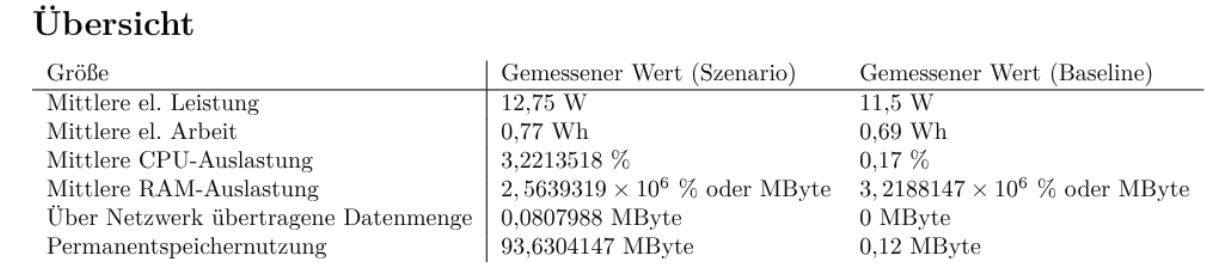
\includegraphics[width=10cm]{../img/OSCAR_example.png}
        \end{figure}

        As shown in the graphic, the power consumption is needed in watts, further OSCAR needs information about CPU, RAM and networing status, what is the reason why 'Collectctl' is used during the emasurement.



        \subsection{Interfaces between used components}
        \subsection{Test the Lab-setup}

    \section{Testing software for it's energy consumption}
        \subsection{Making actual testruns for each scenario}
        \subsection{Process the collected data}

    \section{Appendix}

%     Image 1 - https:\/\/eco.kde.org/be4foss-handbook/images/sec3$_$lab-setup$_$modified.png
%     Image 2 - https://invent.kde.org/teams/eco/feep/-/blob/master/measurements/okular/2022-09-22/Bericht%20OSCAR%20Standardnutzungsszenario.pdf

%     \section{Evaluation}
%         \subsection{Evaluation of the testing scripts}
%         \subsection{Evaluation of the measurement results}

    \newpage

    \begin{center}
    \section*{Rough timeline for project points:}
    \begin{tabular}{ | l | r | }
    \hline
    Task & Deadline \\
    \hline\hline
    1: Get familiar with the project and perform a successful merge request   & Nov \\
    \hline
    2: Evaluate Selenium and learn the important parts of the framework & Dec\\
    \hline
    3: Translation of Ocular, Kate and LibreOffice to Selenium & Feb\\
    \hline
    4: Setup Testing Lab & Mar\\
    \hline
    5: Test software's energy consumption & Apr\\
    \hline
    6: Evalutaion & May\\
    \hline
    \end{tabular}
    \end{center}

    \begin{center}
    \section*{Weekly Schedule}
    \begin{tabular}{ | c | c | c | }
    \hline
    Week & Task & Meeting \\
    \hline\hline
    41  & Setup fedora VM (with KDE Plasma) and ydotool/kdotool & y \\
    \hline
    42  & Setup the project locally and and test the local setup/run and test scripts & y \\
    \hline
    43  & Change something and perform first merge request to the repository & y \\
    \hline
    44  & Write introduction to the topic (chapter 1) & \\
    \hline
    45  & Write introduction to the topic (chapter 1) & \\
    \hline
    46  & Learn Selenium, AT-SPI and needed components & y \\
    \hline
    47  & Setup Selenium, AT-SPI & \\
    \hline
    48  &  Setup Selenium, AT-SPI & y \\
    \hline
    49  &  Write and test first Selenium scripts & \\
    \hline
    50  &  Translation Okular to Selenium - baseline, idle & y \\
    \hline
    51  & Translation Okular to Selenium - sus & \\
    \hline
    52  & Translation Okular to Selenium - sus; Test the scripts, evaluation with team & \\
    \hline
    53  & buffer & \\
    \hline
    1  & Translation Kate to Selenium - baseline, idle & y \\
    \hline
    2  & Translation Kate to Selenium - sus & \\
    \hline
    3  & Translation Kate to Selenium - sus; Test the scripts, evaluation with team & y \\
    \hline
    4  & Write thesis & \\
    \hline
    5  & Write thesis & \\
    \hline
    6  & Plan Lab - create checklist & ? \\
    \hline
    7  & (Holidays - school closed): Plan Lab, write thesis &  \\
    \hline
    8  & Setup and Test Lab - troubleshooting &  \\
    \hline
    9  & Setup and Test Lab - troubleshooting & ? \\
    \hline
    10  & Perform tests for each of the three scenarios & \\
    \hline
    11  & Perform tests for each of the three scenarios & ? \\
    \hline
    12  & ?Perform tests?/Process test data & \\
    \hline
    13 & Evaluate tests & ? \\
    \hline
    14 & Write thesis & \\
    \hline
    15 & Eventually: scripts for new applications??? & \\
    \hline
    tba & tba & tba \\
    \hline

    \end{tabular}
    \end{center}

    \begin{lstlisting}[language=Python]
    import numpy as np

    def incmatrix(genl1,genl2):
        m = len(genl1)
        n = len(genl2)
        M = None #to become the incidence matrix
        VT = np.zeros((n*m,1), int)  #dummy variable

        #compute the bitwise xor matrix
        M1 = bitxormatrix(genl1)
        M2 = np.triu(bitxormatrix(genl2),1)

        for i in range(m-1):
            for j in range(i+1, m):
                [r,c] = np.where(M2 == M1[i,j])
                for k in range(len(r)):
                    VT[(i)*n + r[k]] = 1;
                    VT[(i)*n + c[k]] = 1;
                    VT[(j)*n + r[k]] = 1;
                    VT[(j)*n + c[k]] = 1;

                    if M is None:
                        M = np.copy(VT)
                    else:
                        M = np.concatenate((M, VT), 1)

                    VT = np.zeros((n*m,1), int)

        return M
    \end{lstlisting}

    \lstinputlisting[language=Python]{../src/main.py}

\end{document}
